\subsection{\textbf{\uppercase{Customização do Asterisk}}}

A customização do Asterisk será fundamental para realizar a comunicação entre os sistemas, sendo responsável em disponibilizar de forma padronizada o acesso a URA no atendimento de primeiro nível de todas as chamadas recebidas, e disparar solicitações a recursos externos conforme a necessidade do cliente que efetuou a ligação.
Primeiramente foi configurado um ramal, utilizando a interface web do Disc-OS, conforme exemplo a seguir na figura \ref{figura:cadastroRamapSIP}:


\begin{figure}[H]
	\centering
	\caption{\textbf{Cadastro de um Ramal SIP.}}	
	\label{figura:cadastroRamapSIP}
		\begin{subfigure}[H]{\textwidth}
			\centering
			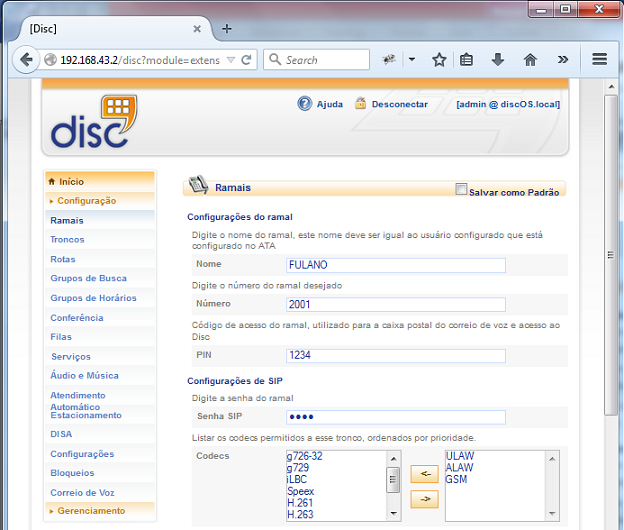
\includegraphics{figuras/cadastro_ramal_sip.png}
		\end{subfigure}
	\\[6pt]
	\fontsize{10}{12}\selectfont {Fonte: Autoria Própria.}
\end{figure}


Conforme visto na figura \ref{figura:cadastroRamapSIP}, está sendo configurado o ramal de número 2001, com o nome de FULANO e definido alguns \textit{codecs} que serão permitidos utilizar neste ramal, após isto o Disc-OS se encarregará de alterar o arquivo de propriedades \textit{sip.conf} inserindo o ramal desejado com as características informadas.
Para a configuração da Unidade de Resposta Audível, será preciso definir claramente quais serão as opções disponíveis e quais serão as possíveis saídas com os seus devidos tratamentos, neste trabalho foi desenvolvido um fluxo de atendimento próprio, demonstrado na figura \ref{figura:fluxoURA}: 

\begin{figure}[H]
%	\centering
	\caption{\textbf{Diagrama do Fluxo da Unidade de Resposta Audível}}
	\label{figura:fluxoURA}	
		\begin{subfigure}[H]{\textwidth}
			\centering
			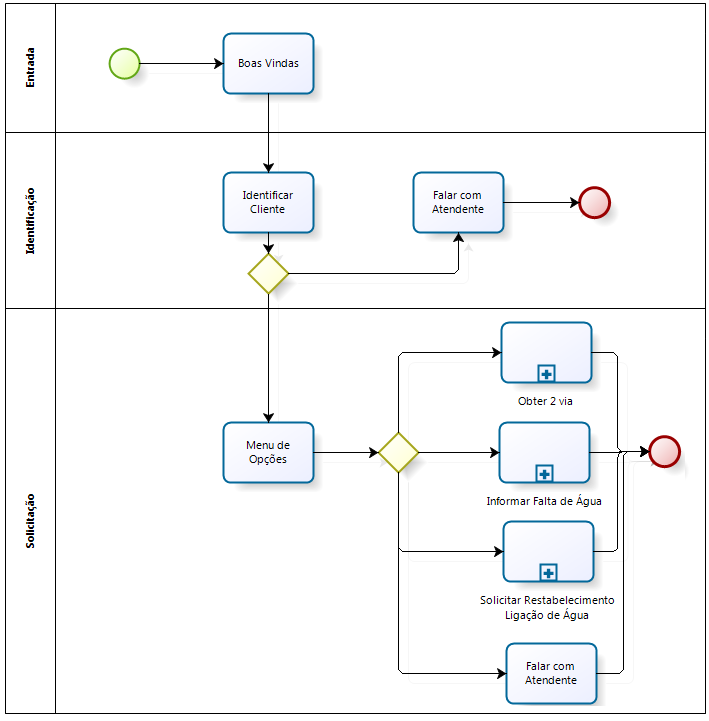
\includegraphics{figuras/fluxo_ura.png}
		\end{subfigure}
	\\[6pt]
	\fontsize{10}{12}\selectfont {Fonte: Autoria Própria.}
\end{figure}


Dessa forma o cliente tem a opção de falar com o atendente logo no primeiro menu de atendimento e nos demais sub fluxos, comportamento exigido conforme o artigo 4 da Lei nº 8.078 \cite{leiAtendimentoAoConsumidor}, que fixa normas gerais sobre o Serviço de Atendimento ao Consumidor, após realizar o passo de identificação o mesmo terá acesso as opções de serviços automatizados via integração caso ocorra tudo com êxito, caso não seja possível identificar o cliente será redirecionado para o Falar com Atendente.
A interface \textit{Web} do Disc-OS permite realizar a configuração da URA, de forma bem intuitiva, inclusive definir tempos de espera, direcionamento para outros Ramais entre outras configurações que tornam o processo de configuração muito mais prático, no entanto para configurar o fluxo da URA realizando a comunicação via AGI com o \textit{Middleware} será preciso realizar o procedimento manual de configuração, segue a configuração utilizada para criação do contexto de PESQUISAR\_CLIENTE utilizada para identificar o cliente, descrito no arquivo \textit{/etc/asterisk/extensions.conf}, conforme representado pela figura \ref{figura:fluxoIdentificacaoClienteAsterisk} a seguir:


% Custom exibição da lista de algoritmos
%\algsetup{
%	linenosize=\small,
%	linenodelimiter=.	
%}

%\begin{algorithm}
%	\caption{Fluxo de identificação do cliente (Asterisk).}	
%	\label{algoritmo:FluxoIdentificaoCliente}
%	\begin{algorithmic}[1]
%		\STATE $atenderLigação()$ \COMMENT{ recepciona a ligação}
%		\STATE $tocarAudio(beep)$   \COMMENT{tocar áudio de aviso}
%		\STATE $tempo\_limite\_discagem \gets 3$  \COMMENT{ defini tempo limite de espera entre dígitos }		 
%		\STATE $tempo\_limite\_resposta \gets 7$  \COMMENT{ defini tempo limite de espera do primeiro digito}
%		\STATE $digitos  \gets lerDigitos()$  \COMMENT{ ler os dígitos informados }
%		\STATE $canal [cliente]  \gets digitos$   \COMMENT{ adiciona os dígitos no canal  }
%		\STATE $Agi(pesquisar.imovel.cliente.agi)$  \COMMENT{ faz a chamada agi }
%		\IF { $canal [situacao] == 'sucesso'$ }
%		\STATE $gotoSucesso()$  \COMMENT{ redireciona a ligação para sucesso }
%		\ELSE
%		\STATE $ gotoContextoAtendente()$  \COMMENT{ redireciona a ligação para falar com atendente	}
%		\ENDIF		
%	\end{algorithmic}
%\end{algorithm}


\begin{figure}[H]
	%\centering
	\caption{\textbf{Fluxo de Identificação de Cliente no Asterisk.}}	
	\label{figura:fluxoIdentificacaoClienteAsterisk}
	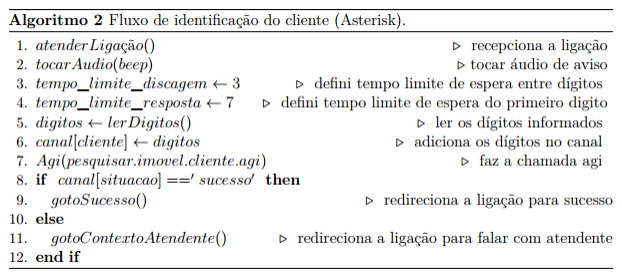
\includegraphics{figuras/algoritmo_2.png}
	\\[6pt]
	\fontsize{10}{12}\selectfont {Fonte: Autoria Própria.}
\end{figure}

A figura \ref{figura:fluxoIdentificacaoClienteAsterisk} acima representa a rotina que será executada toda vez que um cliente ao entrar em contato com a Central de Atendimento e optar em se identificar, ao selecionar essa opção a URA por meio do contexto [PESQUISAR\_CLIENTE] irá anteder a ligação e logo em seguida emitir um áudio chamado \textit{"beep"}, após este som o cliente terá 7 segundos para informar o primeiro dígito e 3 segundos de esperar entre os dígitos, quanto o cliente terminar de informar os dígitos de identificação o algoritmo irá atribuir os dígitos à variável chamada CLIENTE\_IMOVEL e realizar o processo de requisição via interface de comunicação AGI para o \textit{Middleware}, solicitando o serviço mapeando em "pesquisar.imovel.cliente.agi", caso o cliente seja identificado com sucesso a ligação será direcionada para o contexto de opções dos serviços automatizados, caso contrário a ligação será redirecionada para o atendente.

O fluxo de atendimento da URA, permite que seja configurado um arquivo de Áudio para interação com o cliente, neste trabalho foram criados os arquivos de áudio para serem tocados, conforme as operações disponíveis forem acessadas.
A própria ferramenta Asterisk fornece uma forma de gravar um arquivo de áudio, discando para o número *77 é acionado um aplicativo nativo que começa a gravar oque for falado na chamada após o termino da chamada é salvo o arquivo de áudio no diretório \textit{/var/lib/asterisk/sounds/custom/} para utilização.
 
Após as configurações básicas, é preciso ter um dispositivo para efetuar as chamadas e conseguir se comunicar com a URA, neste cenário existe um recurso chamado de \textit{Softphone}, são programas que tornam o computador em um Ramal IP, possibilitando realizar e receber chamadas, com essa finalidade foi utilizado o Zoiper\footnote{Zoiper - Softphone que fornece recursos para simular ramais}.

Para adicionar o ramal é preciso definir qual será o protocolo utilizado e inserir os dados configurados no Asterisk conforme visto na figura \ref{figura:zoiperConfigRamal} abaixo:

\begin{figure}[H]
	%\centering
	\caption{\textbf{Configurar Ramal no Zoiper}}
	\label{figura:zoiperConfigRamal}
	\begin{subfigure}[H]{\textwidth}
		\centering
		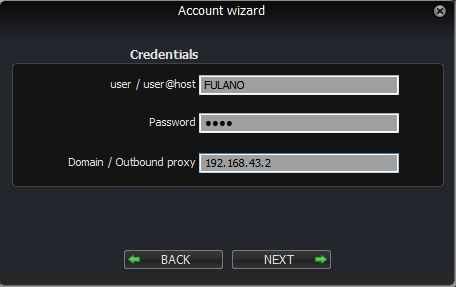
\includegraphics{figuras/configurar_ramal_zoiper.png}
	\end{subfigure}
	\\[6pt]
	\fontsize{10}{12}\selectfont {Fonte: Autoria Própria}.
\end{figure}


Após realizar todos estes passos é possível acessar os serviços disponibilizados pela URA, através do Zoiper efetuar as chamadas para percorrer os fluxos previamente definidos.